\section{Introduction}
I have spent the majority of my time this week having a look at tasks from MultiMediaEval 2018\cite{mediaeval18}, examining the dataset and considering appropriate strategies.

\section{Medico Multimedia\cite{medico18}}
\subsection{Description}
The Medico Task tackled the challenge of predicting diseases based on multi-media data collected in hospitals with two additional requirements: perform the analysis efficiently and use as little data as possible for training.

Beside the 2 main tasks there were 2 more optional subtasks which were basic reporting required built system to generate summarization of a video in terms of how many different diseases and findings have occurred (e.g. if the same polyp occurs twice it should only be counted one time for the summary); and advanced reporting required the built system to automatically create a text-report for a physician for three video cases.

\subsection{Dataset}
{MediaEval provided 2 different datasets which were \textbf{\emph{{Medico-2018-develop-ment-set}}} and \textbf{\emph{Medico-2018-development-set-features}}.

The first one was the image-type dataset to work with, containing 5293 images with multiple resolutions, 16 classes. The image files were encoded using JPEG compression\cite{jpeg}, extension of the image files was ".jpg". 

The second one contained the extracted visual feature descriptors for all the image from the first dataset. The extracted visual features were stored in separate folders and files named accordingly to the name and the path of the corresponding image files. The extracted visual features were the global image features, namely: JCD, Tamura, ColorLayout, EdgeHistogram, Auto-ColorCorrelogram and PHOG. Each feature vector consists of a number of floating point values. The size of the vector depends on the feature. The size of the feature vectors are: 168 (JCD), 18 (Tamura), 33 (Color-Layout), 80 (EdgeHistogram), 256 (AutoColorCorrelogram) and 630 (PHOG). The exten-sion of the extracted visual feature files was ".features".

After examining the dataset I had the result of number of images per class: \textbf{\emph{polyps}} had 613 images, \textbf{\emph{dyed-lifted-polyps}} had 457 images, \textbf{\emph{ulcerative-colitis}} had 457 images, \textbf{\emph{esophagitis}} had 444 images, \textbf{\emph{normal-pylorus}} had 439 images, \textbf{\emph{normal-z-line}} had 437 images, \textbf{\emph{dyed-resection-margins}} had 416 images, \textbf{\emph{normal-cecum}} had 416 images, \textbf{\emph{retroflex-stomach}} had 398 images, \textbf{\emph{stool-plenty}} had 366 images, \textbf{\emph{colon-clear}} had 267 images, \textbf{\emph{retroflex-rectum}} had 237 images, \textbf{\emph{blurry-nothing}} had 176 images, \textbf{\emph{stool-inclusions}} had 130 images, \textbf{\emph{instruments}} had 36 images, \textbf{\emph{out-of-patient}} had 4 images.

\subsection{Models}
\subsubsection{ResNet\cite{resnet}}
My reconfigured ResNet model could be found \href{https://github.com/tlvu2697/mediaeval-18--medico-multimedia}{on my GitHub}.

\section{Emotional Impact of Movies\cite{emotion18}}
\subsection{Description}
There were two types of emotion which were expected emotions and induced emotions. The expected emotion was the emotion which most of the audience feels in  the same context. This type of emotions could be considered objective because it reflected the unanimous response of audiences to a given stimulus \cite{emotion}. On the other hand, induced emotion was subjective and context dependent. In other words, induced emotions were somewhat personal emotions while expected emotions were the general emotions of a population.

\begin{figure}[!ht]
\centering
\begin{subfigure}{0.5\textwidth}
  \centering
  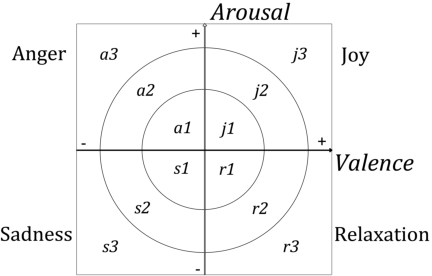
\includegraphics[height=0.17\textheight,keepaspectratio]{week8-emo-valence-arousal.png}
  \caption{Image of Joel Eaton et al.}
\end{subfigure}%
\begin{subfigure}{0.5\textwidth}
  \centering
  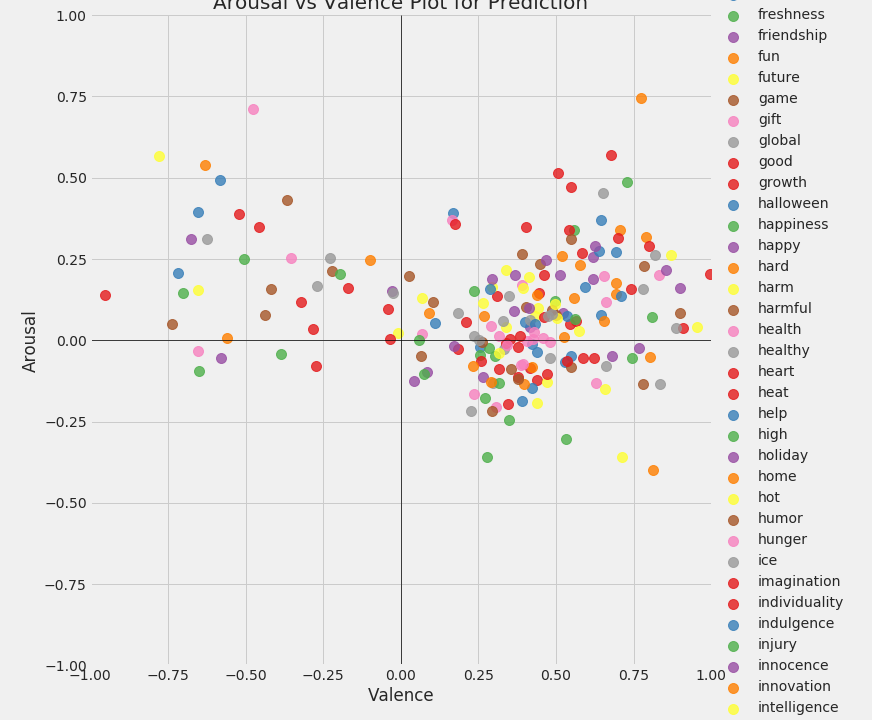
\includegraphics[height=0.18\textheight,keepaspectratio]{week8-emo-types.png}
  \caption{Image of Tejas Mahajan.}
\end{subfigure}
\caption{Expected emotions vs Induced emotions.}
\end{figure}

Moreover, the emotion felt during a movie scene may also depended on the previous emotions as well as scenes. Therefore, temporal information could be used to predict emotions.

In particular, our objective was to predict a score of \textbf{induced valance} (which was the attractiveness (positive valence) or the averseness (negative valence) \cite{valence}) and \textbf{induced arousal} (which was the level of excitement). Va-lence could be negative (e.g. sad, disappointed, etc.) or positive (e.g. joyful, elated, ...). Arousal ranged from inactive (e.g. tired, pensive, calm) to active (e.g. alarmed, angry, excited). Valence and arousal score could be represented as scores from -1 to 1. The expected emotions were then calculated based on these two scores (see figure 7.6). In this task, we would only have to compute the induced emotions scores. The second task of the challenge was fear prediction. We would have to predict and label the beginning and ending times of video sequences that caused fear in movies. The objective of this task was pretty clear so I would continue to the next task of summarizing the dataset.

\subsection{Dataset}
The development set contained 44 movies (durations of 15 hours and 20 minutes) for both subtasks as well as a complementary set of 10 movies (dura-tions of 11 hours and 29 minutes) just for the first subtask. There were audio and video features provided for all videos. Annotations for both subtasks were also available is development set. The test set consisted of 12 movies (total durations of 8 hours and 50 minutes). Neither audio nor video features were provided as the time of this report.

\subsection{Train Set}

\textbf{Audio features}: The audio features were extracted using openSmile too-lbox \cite{opensmile}. There are a total of 1,582 features for each second of the video. All features are stored in \textit{.csv} format.

\textbf{Visual features}: Visual features were also extracted for every second of each video. Each frame was extracted using ffmpeg command: "ffmpeg -loglevel error -i movie.mp4 -r 1 -f image2 frame-\%05d.jpg". Most features were extracted using LIRE library with the exception of vgg16 fc6 output.

This was the list of all provided visual features: Auto Color Correlogram (acc), Color and Edge Directivity Descriptor (cedd), Color Layout (cl), Edge Histogram (eh), Fuzzy Color and Texture Histogram (fcth), Gabor (gabor), Joint descriptor joining CEDD and FCTH in one histogram (jcd), Scalable Color (sc), Tamura (tamura), Local Binary Patterns (lbp), VGG16 fc6 layer output (fc6).

\subsection{Test Set}
At the moment, only the source video are available. There were 12 movies in test set.

\subsection{Evaluation}
Mean Square Error and Pearson correlation coefficient would be used for the Valence/Arousal prediction subtask. And Intersection over Union of time in-tervals would be used for the Fear prediction subtask.


\section{Media Memorability}
\subsection{Description}
The Predicting Media Memorability Task\cite{memo18} required participants to build systems predicting how memorable a video was, by computing a memorability score for each input video.

Beside the main task there were 2 more subtasks which were Short-term Memorability and Long-term Memorability\cite{longtermmem}. The Short-term Memorability subtask involves predicting a short-term memorability score for a given video. The Long-term Memorability subtask involves predicting a long-term memo-rability score for a given video.

\subsection{Dataset}
\subsubsection{Overview}
The dataset was composed of 10,000 short soundless videos (named from video1.webm to video10000.webm); 8,000 elements (randomly picked) for the development set and the other 2,000 elements for the test set.

Each video came with its original title (might be useful to infer the memo-rability of video); its short-term memorability score; the number of annotations which was used to calculate its short-term memorability score; its long-term memorability score; the number of annotations which was used to calculate its long-term memorability score.

\subsubsection{Data}
All 8,000 videos were placed in /source folder and named with format of video\{\}.webm; their original titles were placed in dev-set\_video-captions.txt. Each video was 7 seconds long and soundless.

\begin{figure}[!ht]
\centering
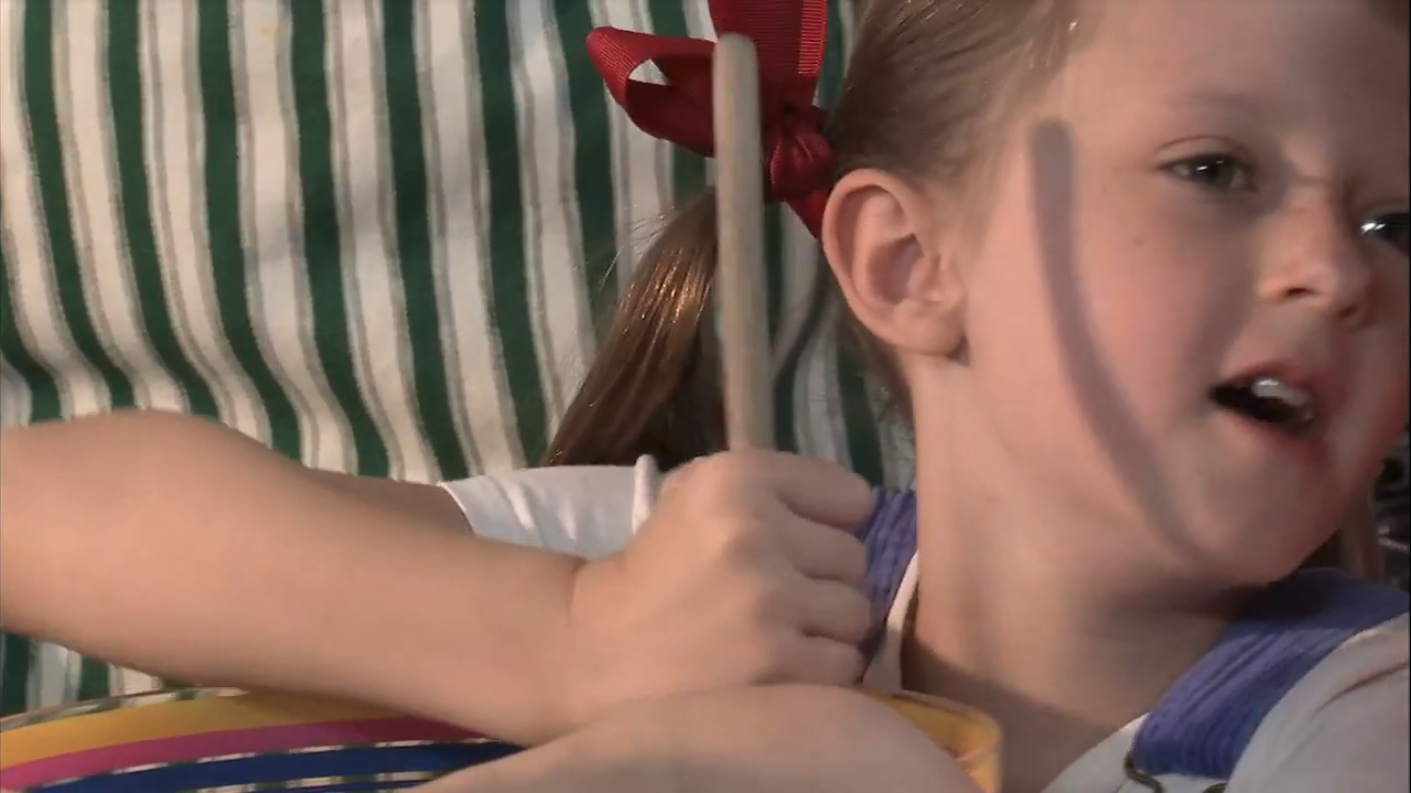
\includegraphics[width=0.8\textwidth]{week8-me-mo-video124.png}
\caption{video124 -- children-help-their-mother-mix-ingredients}
\end{figure}

\begin{figure}[!ht]
\centering
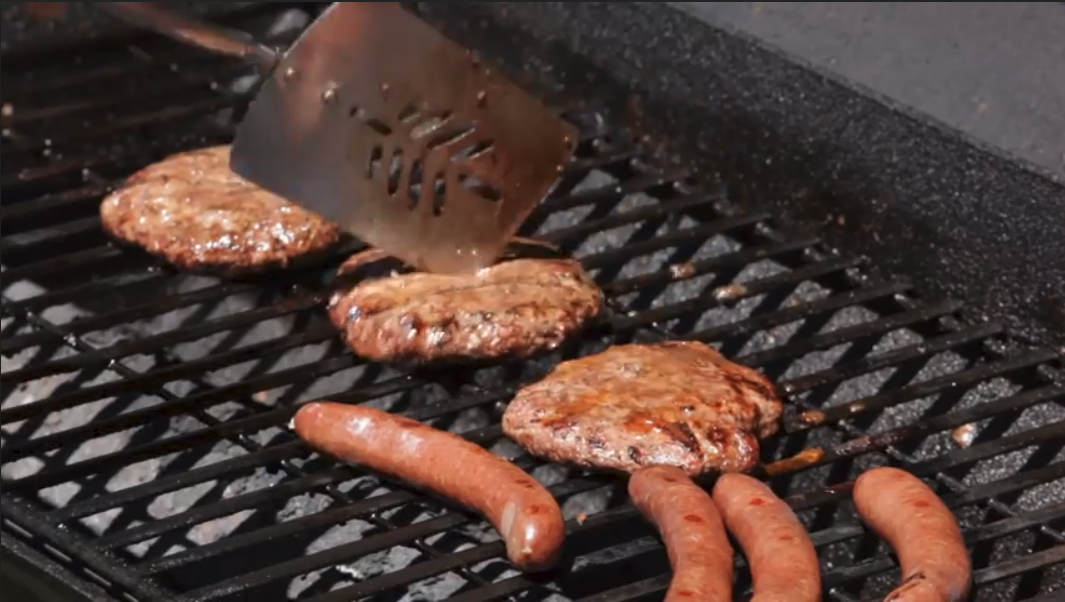
\includegraphics[width=0.8\textwidth]{week8-me-mo-video9740.png}
\caption{video9740 -- flipping-meat-on-grill}
\end{figure}

\subsubsection{Ground Truth}
The videos came with initial memorability scores, defined as the percentage of correct detections by participants, for both short-term and long-term memory performances.

\begin{figure}[!ht]
\centering
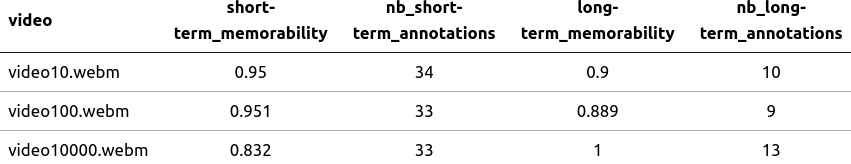
\includegraphics[width=\textwidth]{week8-me-mo-groundtruth.png}
\caption{Example of provided Ground Truth}
\end{figure}

\subsubsection{Pre-computed Features}
There were also total 7 pre-computed content descriptors in 2 different types which were video-dedicated feature and frame-based feature.

\textbf{\emph{Video-decicated feature}}.

\emph{C3D spatio-temporal visual features}\cite{c3d}, obtained by extracting the output of the final classification layer of the C3D model was trained on UCF101 dataset\cite{ucf101} (101 action categories), a 3-dimensional convolutional network proposed for generic video analysis; structured in a single list of numbers (dimension = 101).

\emph{HMP}\cite{hmp}, the histogram of motion patterns for each video; structured in a single list of pairs of numbers with format: bin:number (dimension = 6075).

\textbf{\emph{Frame-based feature}} (extracted on three key-frames - first, middle and last frames).

\emph{HoG descriptors} (Histograms of Oriented Gradients)\cite{hog}, calculated on 32x32 windows on a grey scale version of each frame; structured in single list of numbers on one line (dimension = depends on the image size).

\emph{LBP} (Local Binary Patterns)\cite{lbp}, calculated for patches of 8x15 pixels; structured in a single list of numbers on one line (dimension = depends on the image size).

\emph{InceptionV3 features}\cite{fc7layer}, correspond to the output of the fc7 layer of the InceptionV3 deep network; structured in a single list of pairs of numbers with format imagenet-class:activation (max dimension = 1,000).

\emph{ORB features}\cite{orb}, resulted from a fusion of FAST keypoint detector and BRIEF descriptor; structured in a list of keypoints and descriptors\cite{keypoints}.

\emph{Color histograms}, computed in the HSV space; structured in 3 lists (Red, Green, Blue) of 255 pairs with format bin:number.

These pre-computed features first seemed to be helpful but all of its concepts were so old compared to the year of 2018. And because the purpose of these pre-trained features was to facilitate participation from various communities so they all seemed to be not so useful for us.

\subsubsection{Evaluation}
The official evaluation metric for both subtasks would be the Spearman's rank correlation between the predicted memorability scores and the ground-truth memorability scores.